% Options for packages loaded elsewhere
% Options for packages loaded elsewhere
\PassOptionsToPackage{unicode}{hyperref}
\PassOptionsToPackage{hyphens}{url}
\PassOptionsToPackage{dvipsnames,svgnames,x11names}{xcolor}
%
\documentclass[
  letterpaper,
  DIV=11,
  numbers=noendperiod]{scrartcl}
\usepackage{xcolor}
\usepackage{amsmath,amssymb}
\setcounter{secnumdepth}{-\maxdimen} % remove section numbering
\usepackage{iftex}
\ifPDFTeX
  \usepackage[T1]{fontenc}
  \usepackage[utf8]{inputenc}
  \usepackage{textcomp} % provide euro and other symbols
\else % if luatex or xetex
  \usepackage{unicode-math} % this also loads fontspec
  \defaultfontfeatures{Scale=MatchLowercase}
  \defaultfontfeatures[\rmfamily]{Ligatures=TeX,Scale=1}
\fi
\usepackage{lmodern}
\ifPDFTeX\else
  % xetex/luatex font selection
\fi
% Use upquote if available, for straight quotes in verbatim environments
\IfFileExists{upquote.sty}{\usepackage{upquote}}{}
\IfFileExists{microtype.sty}{% use microtype if available
  \usepackage[]{microtype}
  \UseMicrotypeSet[protrusion]{basicmath} % disable protrusion for tt fonts
}{}
\makeatletter
\@ifundefined{KOMAClassName}{% if non-KOMA class
  \IfFileExists{parskip.sty}{%
    \usepackage{parskip}
  }{% else
    \setlength{\parindent}{0pt}
    \setlength{\parskip}{6pt plus 2pt minus 1pt}}
}{% if KOMA class
  \KOMAoptions{parskip=half}}
\makeatother
% Make \paragraph and \subparagraph free-standing
\makeatletter
\ifx\paragraph\undefined\else
  \let\oldparagraph\paragraph
  \renewcommand{\paragraph}{
    \@ifstar
      \xxxParagraphStar
      \xxxParagraphNoStar
  }
  \newcommand{\xxxParagraphStar}[1]{\oldparagraph*{#1}\mbox{}}
  \newcommand{\xxxParagraphNoStar}[1]{\oldparagraph{#1}\mbox{}}
\fi
\ifx\subparagraph\undefined\else
  \let\oldsubparagraph\subparagraph
  \renewcommand{\subparagraph}{
    \@ifstar
      \xxxSubParagraphStar
      \xxxSubParagraphNoStar
  }
  \newcommand{\xxxSubParagraphStar}[1]{\oldsubparagraph*{#1}\mbox{}}
  \newcommand{\xxxSubParagraphNoStar}[1]{\oldsubparagraph{#1}\mbox{}}
\fi
\makeatother


\usepackage{longtable,booktabs,array}
\usepackage{calc} % for calculating minipage widths
% Correct order of tables after \paragraph or \subparagraph
\usepackage{etoolbox}
\makeatletter
\patchcmd\longtable{\par}{\if@noskipsec\mbox{}\fi\par}{}{}
\makeatother
% Allow footnotes in longtable head/foot
\IfFileExists{footnotehyper.sty}{\usepackage{footnotehyper}}{\usepackage{footnote}}
\makesavenoteenv{longtable}
\usepackage{graphicx}
\makeatletter
\newsavebox\pandoc@box
\newcommand*\pandocbounded[1]{% scales image to fit in text height/width
  \sbox\pandoc@box{#1}%
  \Gscale@div\@tempa{\textheight}{\dimexpr\ht\pandoc@box+\dp\pandoc@box\relax}%
  \Gscale@div\@tempb{\linewidth}{\wd\pandoc@box}%
  \ifdim\@tempb\p@<\@tempa\p@\let\@tempa\@tempb\fi% select the smaller of both
  \ifdim\@tempa\p@<\p@\scalebox{\@tempa}{\usebox\pandoc@box}%
  \else\usebox{\pandoc@box}%
  \fi%
}
% Set default figure placement to htbp
\def\fps@figure{htbp}
\makeatother





\setlength{\emergencystretch}{3em} % prevent overfull lines

\providecommand{\tightlist}{%
  \setlength{\itemsep}{0pt}\setlength{\parskip}{0pt}}



 


\KOMAoption{captions}{tableheading}
\makeatletter
\@ifpackageloaded{caption}{}{\usepackage{caption}}
\AtBeginDocument{%
\ifdefined\contentsname
  \renewcommand*\contentsname{Table of contents}
\else
  \newcommand\contentsname{Table of contents}
\fi
\ifdefined\listfigurename
  \renewcommand*\listfigurename{List of Figures}
\else
  \newcommand\listfigurename{List of Figures}
\fi
\ifdefined\listtablename
  \renewcommand*\listtablename{List of Tables}
\else
  \newcommand\listtablename{List of Tables}
\fi
\ifdefined\figurename
  \renewcommand*\figurename{Figure}
\else
  \newcommand\figurename{Figure}
\fi
\ifdefined\tablename
  \renewcommand*\tablename{Table}
\else
  \newcommand\tablename{Table}
\fi
}
\@ifpackageloaded{float}{}{\usepackage{float}}
\floatstyle{ruled}
\@ifundefined{c@chapter}{\newfloat{codelisting}{h}{lop}}{\newfloat{codelisting}{h}{lop}[chapter]}
\floatname{codelisting}{Listing}
\newcommand*\listoflistings{\listof{codelisting}{List of Listings}}
\makeatother
\makeatletter
\makeatother
\makeatletter
\@ifpackageloaded{caption}{}{\usepackage{caption}}
\@ifpackageloaded{subcaption}{}{\usepackage{subcaption}}
\makeatother
\usepackage{bookmark}
\IfFileExists{xurl.sty}{\usepackage{xurl}}{} % add URL line breaks if available
\urlstyle{same}
\hypersetup{
  colorlinks=true,
  linkcolor={blue},
  filecolor={Maroon},
  citecolor={Blue},
  urlcolor={Blue},
  pdfcreator={LaTeX via pandoc}}


\author{}
\date{}
\begin{document}


\subsection{}\label{section}

{MACHINE LEARNING} {\&} {CAUSALITY}

{The Impact of Financial Crises on Growth}

{--- and where the field has gone since}

{Andrew Tiffin}

{IMF Working Paper 19/228 \textbar{} Updated March 2026}

\begin{center}\rule{0.5\linewidth}{0.5pt}\end{center}

\subsection{}\label{section-1}

{\emph{``The difficulty is to detach the framework of fact --- of
absolute fact ---}}

{\emph{from the embellishments of theorists\ldots``}}

{--- The Memoirs of Sherlock Holmes}

\begin{center}\rule{0.5\linewidth}{0.5pt}\end{center}

\subsection{The Core Tension}\label{the-core-tension}

\begin{center}
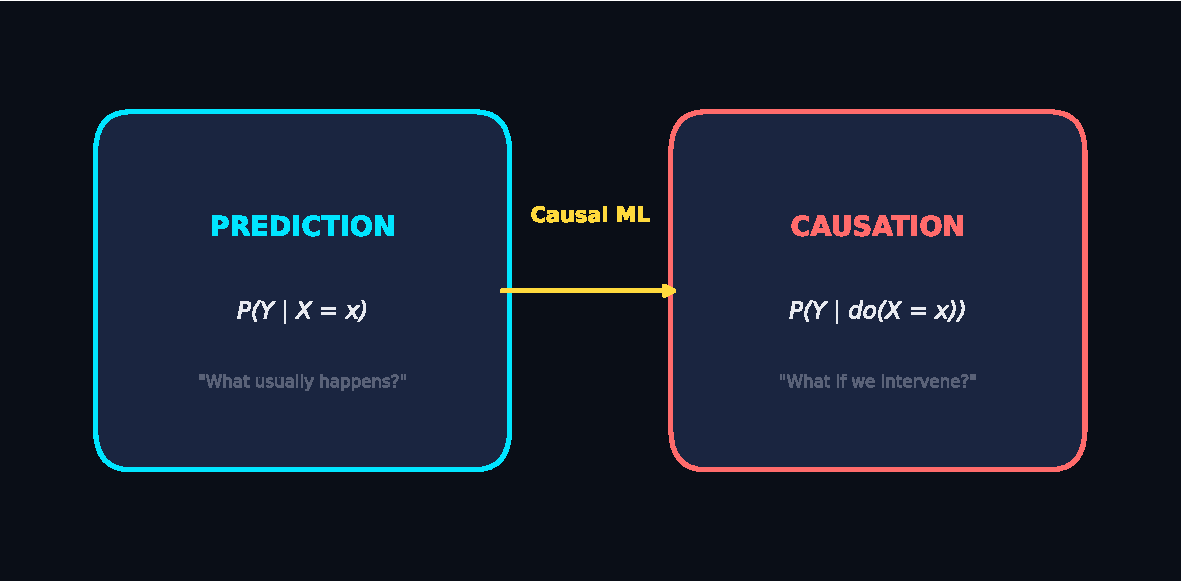
\includegraphics[width=0.8\linewidth,height=\textheight,keepaspectratio]{ml_causality_deck_files/mediabag/deck_assets/07_pred_vs_cause.pdf}
\end{center}

A crowing rooster is a good \textbf{predictor} of sunrise. But
intervening on the rooster won't stop the sun from rising.

\begin{center}\rule{0.5\linewidth}{0.5pt}\end{center}

\subsection{We Never See the Path Not
Taken}\label{we-never-see-the-path-not-taken}

\begin{center}
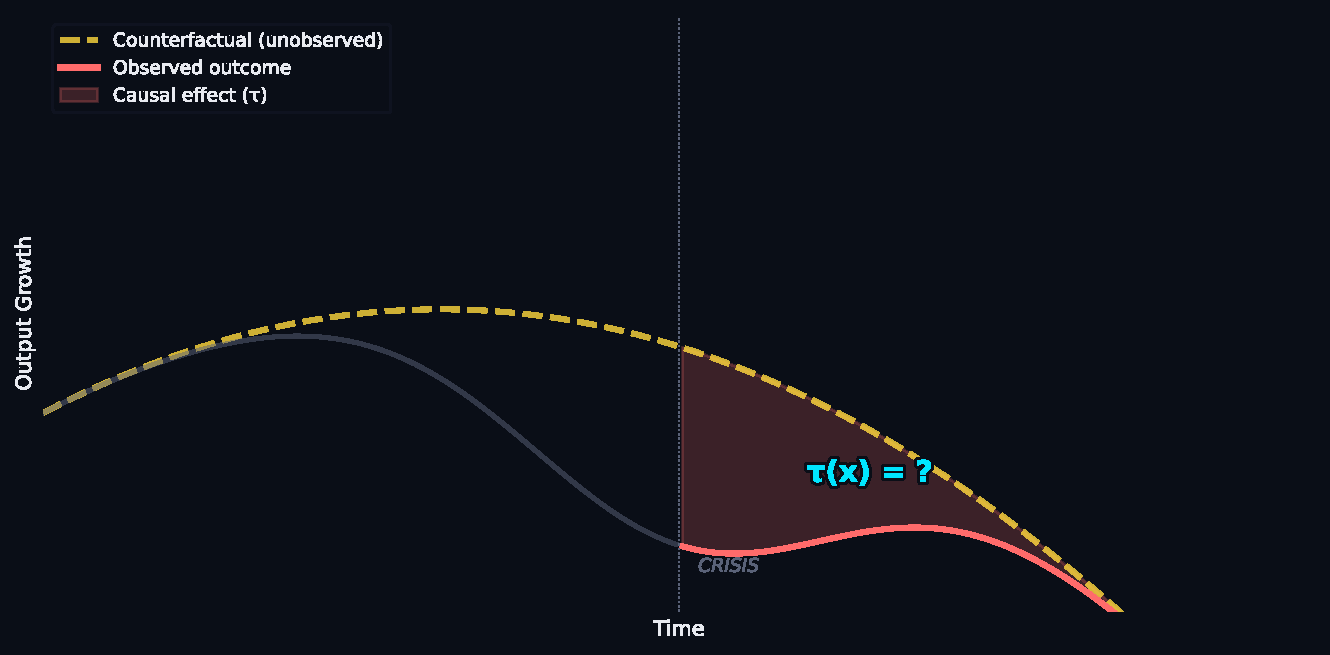
\includegraphics[width=0.85\linewidth,height=\textheight,keepaspectratio]{ml_causality_deck_files/mediabag/deck_assets/01_counterfactual.pdf}
\end{center}

{The \textbf{fundamental problem} of causal inference: we observe one
outcome per unit.}

{Counterfactual predictions can never be validated --- we need them to
be \textbf{plausible}.}

\begin{center}\rule{0.5\linewidth}{0.5pt}\end{center}

\subsection{Why ML Changes the Game}\label{why-ml-changes-the-game}

{CONFOUNDER SELECTION}

LASSO selects which controls matter from hundreds of candidates. Double
selection (Belloni et al., 2014) selects on \textbf{both} outcome and
treatment.

{COUNTERFACTUAL QUALITY}

ML propensity scores build better matches between treated and control
groups. Better E{[}Y\textbar X{]} directly improves counterfactual
estimates.

{HETEROGENEOUS EFFECTS}

\textbf{Causal Forests} find who benefits and who is harmed ---
nonparametrically. No need to pre-specify interactions or functional
forms.

\begin{center}\rule{0.5\linewidth}{0.5pt}\end{center}

\subsection{The Average Hides
Everything}\label{the-average-hides-everything}

{THE OLD QUESTION}

\emph{``Does the drug work?''}

One number for everyone. A single average treatment effect.

If the drug helps some patients and harms others, the average may be
\textbf{zero} --- and we'd conclude it doesn't work.

{THE NEW QUESTION}

\emph{``For whom does it work, and why?''}

A \textbf{personalised} effect for each patient --- based on their
characteristics.

We want to know: young patients benefit, elderly patients don't.
\textbf{That's the signal.}

{A \textbf{causal forest} is a machine that answers the new question.}

\begin{center}\rule{0.5\linewidth}{0.5pt}\end{center}

\subsection{How a Causal Forest
Thinks}\label{how-a-causal-forest-thinks}

Imagine sorting patients into groups where the drug's effect is most
\textbf{different}:

{1.} \textbf{Split} the data: find the characteristic that best
separates \emph{who benefits} from \emph{who doesn't} --- age? income?
blood pressure? The algorithm searches, you don't have to guess.

{2.} \textbf{Keep splitting} to maximise the difference in treatment
effects \textbf{between} groups. Each final leaf contains similar people
--- a mini-experiment with its own effect estimate.

{3.} \textbf{Repeat} hundreds of times with random subsets of data and
variables. Average across all trees. The forest is \textbf{robust} where
any single tree is fragile.

{4.} \textbf{Honesty trick}: one half of the data decides \emph{where to
split}; the other half \emph{measures the effect}. This prevents
overfitting and gives valid confidence intervals.

\begin{center}\rule{0.5\linewidth}{0.5pt}\end{center}

\subsection{The Formal Idea}\label{the-formal-idea}

\[Y_i = \tau_{(i)} W_i + X_i \beta + \varepsilon_i\]

{where \(\tau_{(i)}\) is the treatment effect for unit \(i\) --- and it
\textbf{varies}}

{\textbf{Standard regression}: you choose the interactions}

{\textbf{Causal forest}: the algorithm finds them}

{KEY PROPERTIES}

Splits maximise \textbf{heterogeneity of effects} between groups --- not
prediction accuracy.

Each leaf is a neighbourhood of \textbf{similar people}, yielding a
local treatment effect with a valid confidence interval.

No functional form assumed.

\begin{center}\rule{0.5\linewidth}{0.5pt}\end{center}

\subsection{}\label{section-2}

{APPLICATION}

{What is the cost of a}

{financial crisis?}

{107 countries \textbar{} 46 variables \textbar{} 1985--2017}

\begin{center}\rule{0.5\linewidth}{0.5pt}\end{center}

\subsection{Risk vs.~Vulnerability}\label{risk-vs.-vulnerability}

{RISK}

The probability that a crisis occurs. Most EWS models focus here.
\emph{Will the storm hit?}

{VULNERABILITY}

The cost of a crisis, \textbf{if} it occurs. This paper focuses here.
\emph{How sturdy is the house?}

{Two houses on the Florida seaboard face the same \textbf{risk}. A
concrete house is less \textbf{vulnerable} than a wooden one.}

\begin{center}\rule{0.5\linewidth}{0.5pt}\end{center}

\subsection{The Cost Varies
Enormously}\label{the-cost-varies-enormously}

\begin{center}
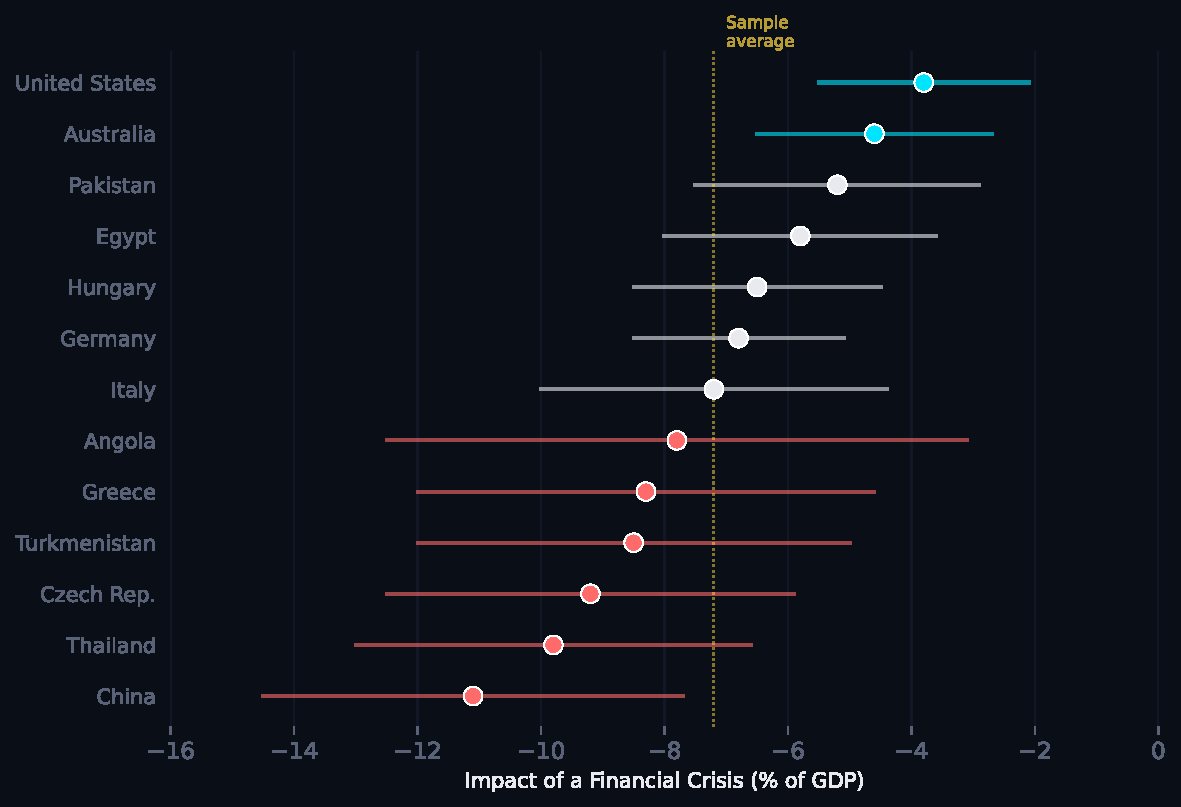
\includegraphics[width=0.75\linewidth,height=\textheight,keepaspectratio]{ml_causality_deck_files/mediabag/deck_assets/02_country_effects.pdf}
\end{center}

{Sample average: \textbf{-7.2 pp} of GDP over two years}

{But ranges from \textbf{-3.8} (United States) to \textbf{-11.1}
(China)}

\begin{center}\rule{0.5\linewidth}{0.5pt}\end{center}

\subsection{Decomposing the Black Box}\label{decomposing-the-black-box}

\begin{center}
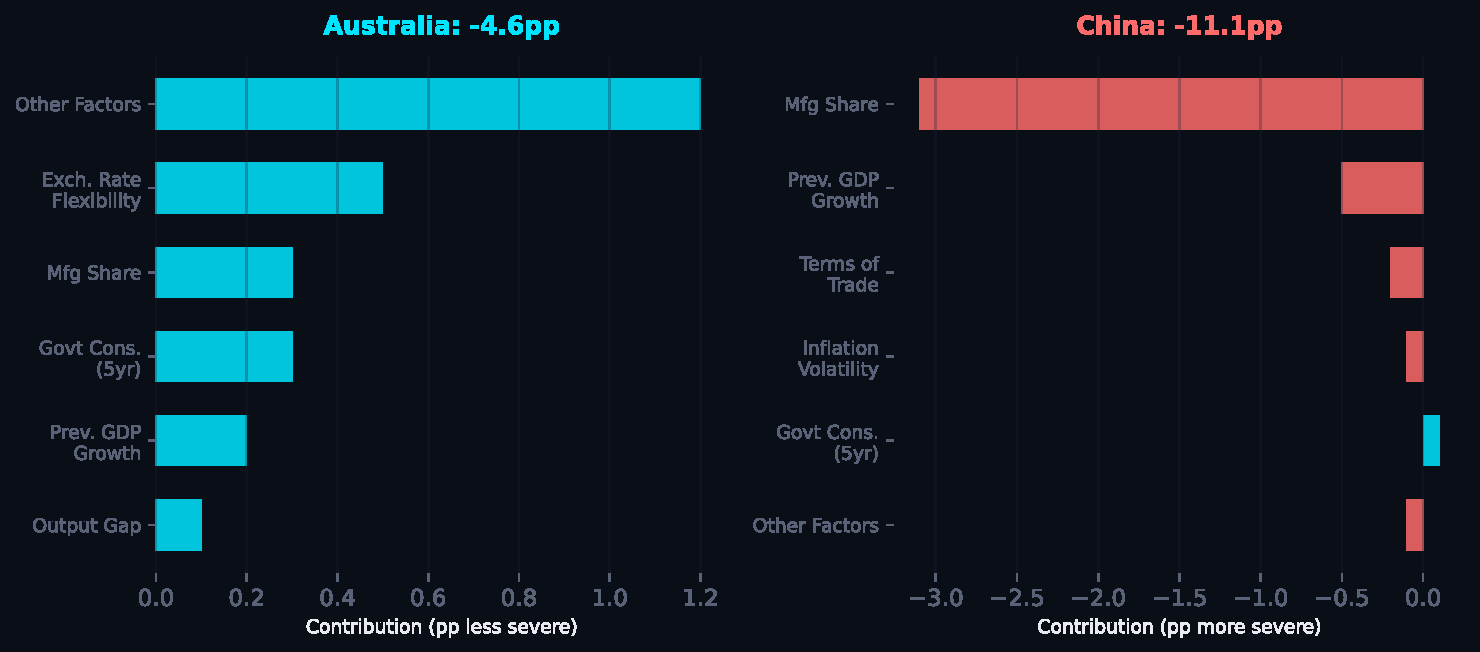
\includegraphics[width=0.9\linewidth,height=\textheight,keepaspectratio]{ml_causality_deck_files/mediabag/deck_assets/03_shapley_waterfall.pdf}
\end{center}

{Shapley values decompose each prediction into variable contributions}

{Australia: flexible exchange rate \textbf{buffers}. China:
manufacturing share \textbf{amplifies}.}

\begin{center}\rule{0.5\linewidth}{0.5pt}\end{center}

\subsection{What Matters Most?}\label{what-matters-most}

\begin{center}
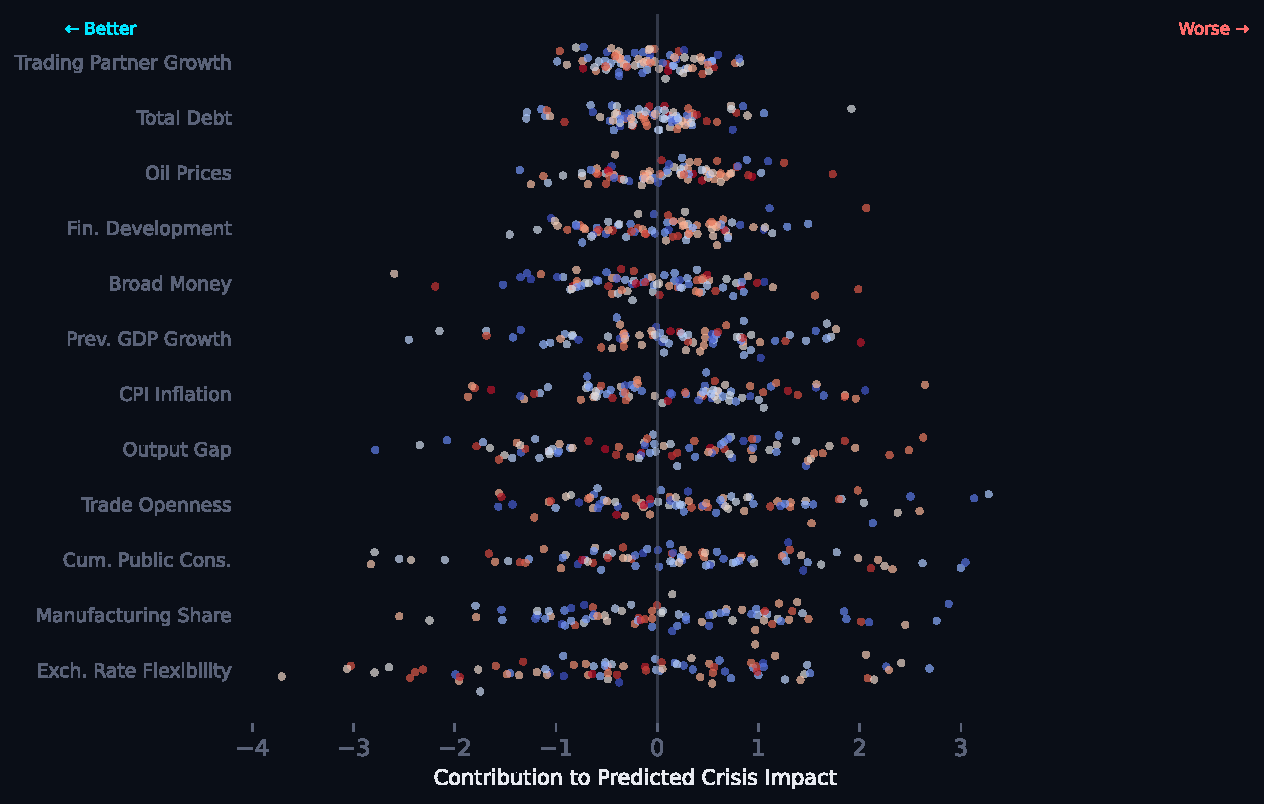
\includegraphics[width=0.85\linewidth,height=\textheight,keepaspectratio]{ml_causality_deck_files/mediabag/deck_assets/04_shapley_distribution.pdf}
\end{center}

{\textbf{Exchange rate flexibility} is the single most important
moderator}

{Variables are ranked by mean \textbar Shapley value\textbar{} --- wider
spread = more important}

\begin{center}\rule{0.5\linewidth}{0.5pt}\end{center}

\subsection{The Exchange Rate Story}\label{the-exchange-rate-story}

\begin{center}
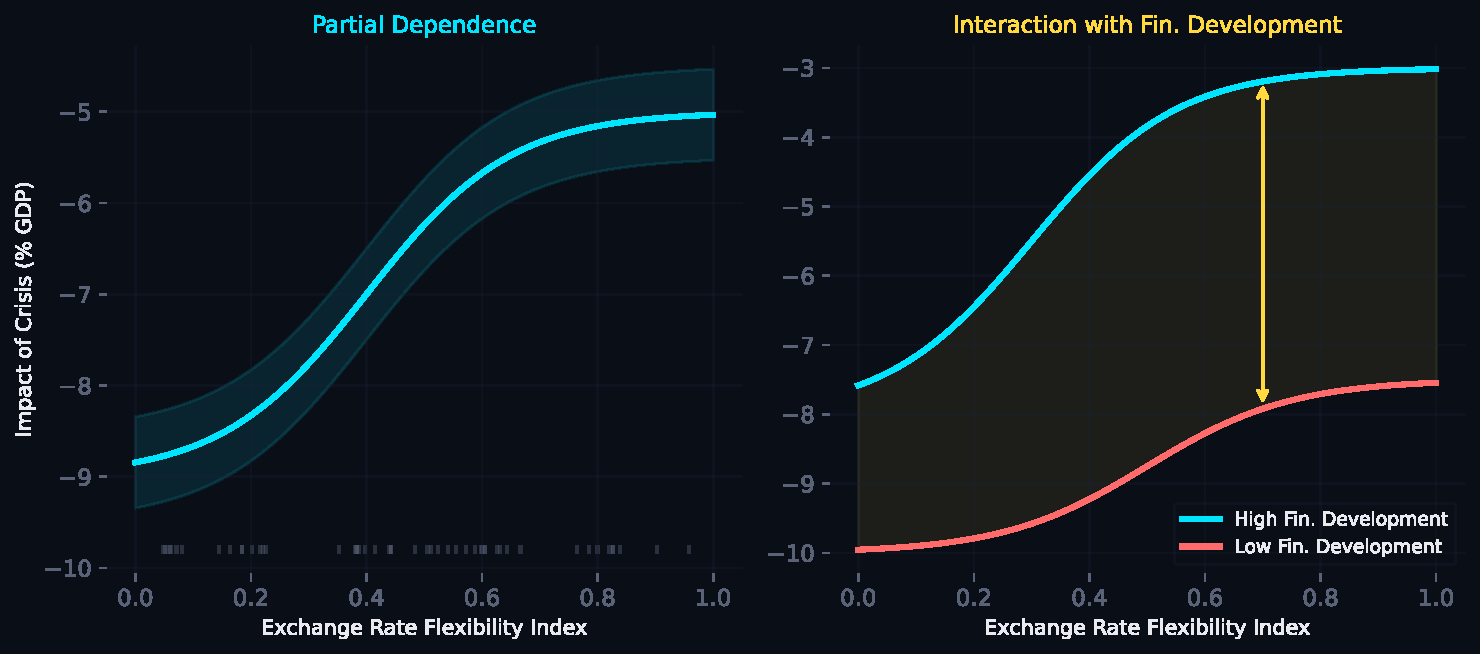
\includegraphics[width=0.9\linewidth,height=\textheight,keepaspectratio]{ml_causality_deck_files/mediabag/deck_assets/05_pdp_interaction.pdf}
\end{center}

{Flexibility reduces crisis cost --- but \textbf{only for financially
developed countries}}

{The interaction is \textbf{nonlinear} --- undetectable by standard
regression}

\begin{center}\rule{0.5\linewidth}{0.5pt}\end{center}

\subsection{}\label{section-3}

{SIX YEARS LATER}

{Where has the}

{field gone?}

\begin{center}\rule{0.5\linewidth}{0.5pt}\end{center}

\subsection{The Causal ML Frontier}\label{the-causal-ml-frontier}

\begin{center}
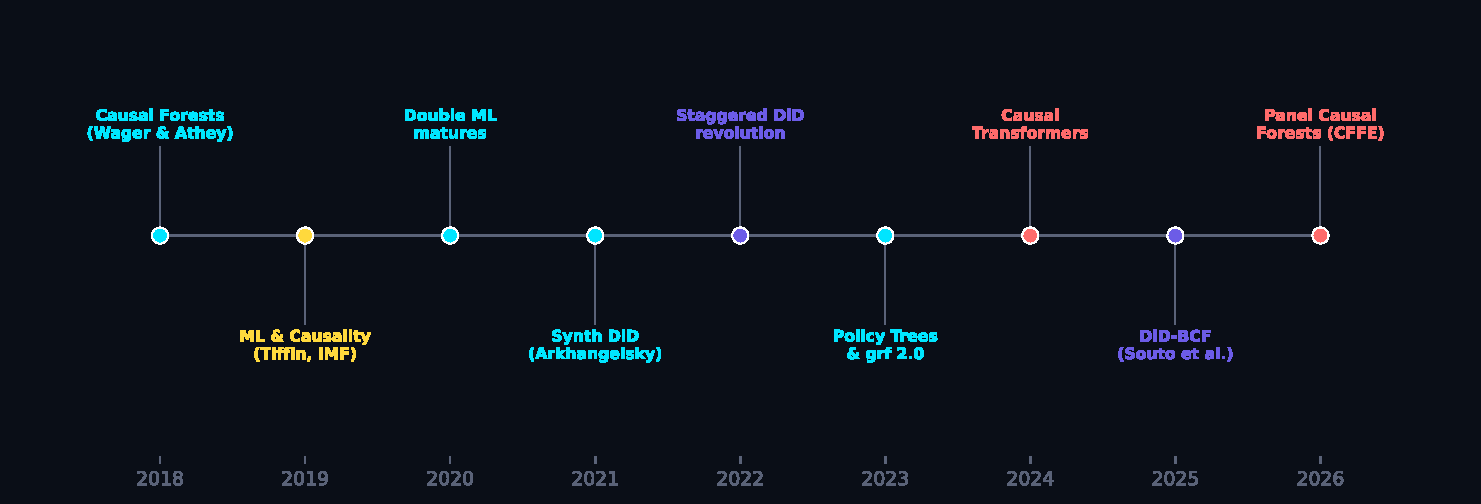
\includegraphics[width=0.95\linewidth,height=\textheight,keepaspectratio]{ml_causality_deck_files/mediabag/deck_assets/06_timeline.pdf}
\end{center}

{From estimating \textbf{average} effects to estimating \textbf{who is
affected and why}}

\begin{center}\rule{0.5\linewidth}{0.5pt}\end{center}

\subsection{The New Toolkit}\label{the-new-toolkit}

{DOUBLE / DEBIASED ML} --- Chernozhukov et al.~(2018)

ML for nuisance parameters + semiparametric efficiency. Clean ATEs in
high dimensions.

{PANEL CAUSAL FORESTS} --- CFFE (Aytug et al., 2026)

Node-level residualisation of fixed effects. HTEs from panel data with
staggered treatment.

{STAGGERED DiD + ML} --- DiD-BCF (Souto et al., 2025)

Bayesian causal forests with parallel trends. Full posterior on CATEs.

{CAUSAL TRANSFORMERS} --- ICML 2026

Cross-attention for long-range confounders. Counterfactuals over time
series.

\begin{center}\rule{0.5\linewidth}{0.5pt}\end{center}

\subsection{What This Paper Would Look Like
Today}\label{what-this-paper-would-look-like-today}

\begin{longtable}[]{@{}
  >{\raggedright\arraybackslash}p{(\linewidth - 2\tabcolsep) * \real{0.5000}}
  >{\raggedright\arraybackslash}p{(\linewidth - 2\tabcolsep) * \real{0.5000}}@{}}
\toprule\noalign{}
\begin{minipage}[b]{\linewidth}\raggedright
2019 Approach
\end{minipage} & \begin{minipage}[b]{\linewidth}\raggedright
2026 Approach
\end{minipage} \\
\midrule\noalign{}
\endhead
\bottomrule\noalign{}
\endlastfoot
Cross-sectional causal forest & \textbf{Panel causal forest (CFFE)} with
unit + time FE \\
SMOTE for class imbalance & \textbf{Honest subsampling} with staggered
treatment timing \\
Shapley values for interpretation & \textbf{SHAP + causal mediation} via
DAG-structured decomposition \\
Single treatment (crisis dummy) & \textbf{Continuous treatment} (crisis
severity) via instrumental forests \\
Post-hoc interaction exploration & \textbf{Policy trees} for optimal
intervention assignment \\
\end{longtable}

{The core insight --- \textbf{heterogeneous vulnerability} --- is more
relevant than ever}

\begin{center}\rule{0.5\linewidth}{0.5pt}\end{center}

\subsection{The Macro Gap}\label{the-macro-gap}

Causal forests have been applied extensively in:

\begin{itemize}
\tightlist
\item
  Labor economics (job training RCTs, wage effects)
\item
  Development economics (education outcomes)
\item
  Health (treatment heterogeneity)
\end{itemize}

But \textbf{barely touched} in:

\begin{itemize}
\tightlist
\item
  Macroeconomic growth
\item
  Trade and industrial policy
\item
  Monetary and fiscal policy transmission
\item
  Resource wealth and TFP
\end{itemize}

{\textbf{The 2019 crisis paper remains one of very few macro
applications.}}

\begin{center}\rule{0.5\linewidth}{0.5pt}\end{center}

\subsection{}\label{section-4}

{KEY TAKEAWAYS}

{1.} {Averages hide everything}

{2.} {Nonlinearities and interactions are the signal, not the noise}

{3.} {The frontier has moved --- but macro hasn't caught up}

{4.} {Panel causal forests are ready for cross-country questions}

\begin{center}\rule{0.5\linewidth}{0.5pt}\end{center}

\subsection{}\label{section-5}

{\emph{``More has been learned about causal inference in the last few
decades}}

{\emph{than the sum total of everything that had been learned about it}}

{\emph{in all prior recorded history.''}}

{--- Gary King, 2007}

{The tools exist. The macro questions are waiting.}




\end{document}
